\documentclass[aspectratio=169,11pt]{beamer}

% Shared style (ib-tutorials.sty at the repo root).
\makeatletter\def\input@path{{./}{../}}\makeatother
\usepackage{ib-tutorials}

\usepackage[utf8]{inputenc}
\usepackage{amsmath,amssymb}
\usepackage{booktabs}
\usepackage{array}
\newcolumntype{L}[1]{>{\raggedright\arraybackslash}p{#1}}
\usepackage{graphicx}
\graphicspath{{../pictures/3-ibamr-fundamentals/}{pictures/3-ibamr-fundamentals/}}
\usepackage{xcolor}
\usepackage{listings}
\usepackage{tikz}
\usetikzlibrary{arrows.meta,positioning,shapes.geometric,fit,calc,decorations.pathmorphing}
\usepackage{hyperref}

\newcommand{\sourcecredit}[1]{\vfill\begin{flushright}\tiny\textcolor{DarkGray}{#1}\end{flushright}}

\lstset{
  basicstyle=\ttfamily\scriptsize\color{BlackGray},
  keywordstyle=\color{NavyBlue}\bfseries,
  commentstyle=\color{DarkGray}\itshape,
  stringstyle=\color{OliveGreen},
  showstringspaces=false,
  columns=fullflexible,
  keepspaces=true,
  breaklines=true,
  breakindent=1em,
  frame=single,
  framerule=0.4pt,
  rulecolor=\color{LightGray},
  backgroundcolor=\color{LightGray!30},
  xleftmargin=0.25em,
  xrightmargin=0.25em
}
\lstdefinestyle{shell}{morecomment=[l]{\#}}
\lstdefinestyle{input}{morecomment=[l]{//}}
\lstdefinestyle{matlab}{morecomment=[l]{\%}}
\lstdefinestyle{python}{morecomment=[l]{\#}}
\lstdefinestyle{data}{}
\lstdefinestyle{tiny}{basicstyle=\ttfamily\tiny\color{BlackGray}}
\lstdefinestyle{inputtiny}{morecomment=[l]{//},basicstyle=\ttfamily\tiny\color{BlackGray}}
\lstdefinestyle{matlabtiny}{morecomment=[l]{\%},basicstyle=\ttfamily\tiny\color{BlackGray}}
\lstdefinestyle{pythontiny}{morecomment=[l]{\#},basicstyle=\ttfamily\tiny\color{BlackGray}}
\lstdefinestyle{shelltiny}{morecomment=[l]{\#},basicstyle=\ttfamily\tiny\color{BlackGray}}
\lstdefinestyle{cpp}{language=C++,morecomment=[l]{//}}
\lstdefinestyle{cpptiny}{language=C++,morecomment=[l]{//},basicstyle=\ttfamily\tiny\color{BlackGray}}

\title[What can go wrong]{What can go wrong, convergence tests and debugging}
\subtitle{The failures of Part III collected and explained, the 2014 troubleshooting rules checked against the code, a convergence study on the bouncing band, and a way of working when a run misbehaves}
\author[Miller]{Laura A. Miller}
\institute[UArizona]{Department of Mathematics, University of Arizona}
\date{Using IB Software \textbullet\ Part III \textbullet\ Chapter 16}

\begin{document}

% 1
\begin{frame}[plain]
\maketutorialtitlepanel{%
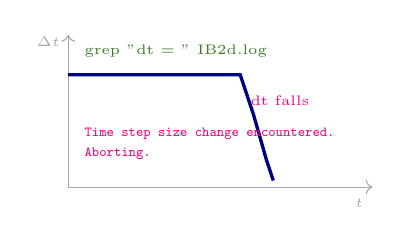
\begin{tikzpicture}[scale=0.84]
  \draw[DarkGray,thin,->] (0,0.3) -- (4.6,0.3); \node[font=\tiny,text=DarkGray] at (4.4,0.05) {$t$};
  \draw[DarkGray,thin,->] (0,0.3) -- (0,2.6); \node[font=\tiny,text=DarkGray] at (-0.3,2.5) {$\Delta t$};
  \draw[NavyBlue,very thick] (0,2.0) -- (2.6,2.0) -- (2.8,1.4) -- (3.0,0.7) -- (3.1,0.4);
  \node[font=\tiny,text=RubineRed] at (3.2,1.6) {\code{dt} falls};
  \node[font=\tiny\ttfamily,text=RubineRed,anchor=west] at (0.1,1.1) {Time step size change encountered.};
  \node[font=\tiny\ttfamily,text=RubineRed,anchor=west] at (0.1,0.8) {Aborting.};
  \node[font=\tiny,text=OliveGreen,anchor=west] at (0.1,2.35) {grep "dt = " IB2d.log};
\end{tikzpicture}}
\end{frame}

% 2
\begin{frame}{Learning goals}
\label{fr:goals}
\footnotesize By the end of this chapter you should be able to:
\begin{enumerate}
  \item recognise the ways an IB simulation fails and read what the program says about it: the CFL abort, a point escaping the box, a parse error, a silent key, a segmentation fault at the first output, a job that the scheduler kills;
  \item apply the 2014 troubleshooting rules (ramp the flow, keep the stiffness down, refine where the vortices are, tighten the solver, match every dimensionless number) and know which of their keys and commands still exist in 0.19.0;
  \item watch a run while it goes, by the time step in the log, and stop it before it wastes a day;
  \item say what convergence, order and stability mean, run the stiff-equation and heat-equation exercises, and carry out a grid-refinement study on an IB example as this chapter does on the bouncing band;
  \item work through a misbehaving run in a fixed order, from the smoke test to the debugger, without guessing.
\end{enumerate}
\begin{punchbox}
\footnotesize Chapters 5--15 each ended with a ``what can go wrong'' slide. This chapter is the union of those, sorted by what you see rather than by where it was found, plus the two things the series had not yet done: a convergence test and a debugging routine.
\end{punchbox}
\end{frame}

% 3
\begin{frame}{How this chapter was checked}
\label{fr:checked}
\begin{itemize}\footnotesize
  \item Every error message quoted is taken from the IBAMR 0.19.0 source (\code{IBHierarchyIntegrator.cpp}, \code{LDataManager.cpp}, \code{ConstraintIBKinematics.cpp}, \code{IBStandardInitializer.cpp}) or from a run of this series, with the chapter where it happened; every input key is one the source reads.
  \item The 2014 tutorial \emph{What can go wrong} (14 slides) is quoted in full and checked line by line: two of its keys, one command and one formula are examined against 0.19.0 (slides \ref{fr:refine}, \ref{fr:tol}, \ref{fr:match}).
  \item The 2021 lecture \emph{Stability and convergence} (MATH 481 Lecture 19, 40 slides) supplies the definitions and the two MATLAB exercises, which this series ships with Python versions (\code{examples/support/matlab-exercises}); its IB2d lab is translated to IBAMR terms.
  \item The convergence study was run for this chapter: IBAMR's \code{examples/IB/explicit/ex1} at four grids, 64 to 512 cells, with the shipped structure files for each, and the band's shape compared across them (slides \ref{fr:conv1}, \ref{fr:conv2}).
  \item The 2019/2020 cluster debugging tips (four slides, UNC's Dogwood) are summarised for Puma; their two inaccuracies are noted.
\end{itemize}
\end{frame}

% 4
\begin{frame}{Where to look things up}
\label{fr:lookup}
\small
\begin{itemize}
  \item \al{The messages}: \code{grep -rn "TBOX\_ERROR" <IBAMR>/src <IBAMR>/ibtk/src} lists every way IBAMR can stop on purpose, with the text it prints; the ones a user meets are on slides \ref{fr:table1} and \ref{fr:table2}.
  \item \al{The time step}: \code{IBHierarchyIntegrator.cpp}, \code{preprocessIntegrateHierarchy} (the dt-change check, keys \code{error\_on\_dt\_change}, \code{warn\_on\_dt\_change}) and \code{postprocessIntegrateHierarchy} (the CFL numbers it logs).
  \item \al{Refinement}: \code{INSHierarchyIntegrator.cpp}, \code{vorticity\_rel\_thresh}, \code{vorticity\_abs\_thresh}; \al{solver tolerances}: \code{INSStaggeredHierarchyIntegrator.cpp} (\code{stokes\_solver\_type}, \code{stokes\_solver\_db}, the PETSc prefix \code{stokes\_}).
  \item \al{This series}: chapter 3 (build and input-file errors), 7 (boundary conditions), 8a and 8b (parameters, dimensionless numbers), 9a--10 (stiffness and time step), 13 (penalty stiffness), 14 (silent keys), 15 (building the upstream examples); IB/01's README has the time-step table.
  \item \al{Sources}: the 2014 \emph{What can go wrong} deck, the 2021 \emph{Stability and convergence} lecture, the 2012 lab ReadMe (slide 5), the 2019 \emph{Debugging tips}.
\end{itemize}
\end{frame}

% 5
\begin{frame}[fragile]{The oldest advice: watch the time step}
\label{fr:dt}
\begin{columns}[T,onlytextwidth]
\begin{column}{0.5\textwidth}
\footnotesize ``The output will be dumped into viz\_IB2d. There will also be some diagnostic info dumped into the file IB2d.log. You will probably want to keep an eye on the timestep size. I do this via \code{\% grep "dt = " IB2d.log} or \code{\% tail -f IB2d.log | grep "dt = "}. If you see that the timestep size decreases dramatically, this usually means that the computation has gone unstable. Reduce the value of `DT' in input2d and restart the model. The timestep size may be too small if the program crashes or the results are very noisy as well.'' (lab ReadMe, 2012, slide 5)
\begin{lstlisting}[style=shelltiny]
# 0.19.0, with enable_logging = TRUE: the same line is still there
$ grep "dt = " IB2d.log | head -3
IBHierarchyIntegrator::advanceHierarchy(): time interval = [0,0.00025], dt = 0.00025
IBHierarchyIntegrator::advanceHierarchy(): time interval = [0.00025,0.0005], dt = 0.00025
IBHierarchyIntegrator::advanceHierarchy(): time interval = [0.0005,0.00075], dt = 0.00025
$ grep -c "At end" run.log        # steps done
$ tail -f run.log | grep "Simulation time"
\end{lstlisting}
\end{column}
\begin{column}{0.48\textwidth}
\footnotesize Thirteen years on this is still the first thing to do. Three refinements:
\begin{itemize}
  \item the step is \emph{fixed} at \code{DT} (or \code{DT\_MAX}) unless the CFL limit \code{cfl}$\,\times\Delta x/|u|_{\max}$ is smaller; in 0.19.0 a step that \emph{changes} is not merely a warning (slide \ref{fr:cfl});
  \item the log also prints the CFL numbers at the end of every step (``CFL number = ...'', the fluid's and the structure's regrid estimates) when logging is on; a CFL number climbing toward \code{CFL\_MAX} is the instability announcing itself;
  \item \code{integral\{F\}} in the screen output (IB/01, chapter 5) is the total Lagrangian force: for a closed structure it should stay at round-off; a growing value is a structure tearing itself apart.
\end{itemize}
\end{column}
\end{columns}
\end{frame}

% 6
\begin{frame}[fragile]{\code{Time step size change encountered}}
\label{fr:cfl}
\begin{lstlisting}[style=cpptiny]
// src/IB/IBHierarchyIntegrator.cpp, preprocessIntegrateHierarchy() (0.19.0)
if (!skip_check_for_dt_change && (d_error_on_dt_change || d_warn_on_dt_change) &&
    !IBTK::rel_equal_eps(dt, d_dt_previous[0]) && !IBTK::rel_equal_eps(new_time, d_end_time))
{
    if (d_error_on_dt_change)
    {
        TBOX_ERROR(d_object_name << "::preprocessIntegrateHierarchy():  Time step size change encountered.\n"
                                 << "Aborting." << std::endl);
    }
    if (d_warn_on_dt_change)
    {
        pout << d_object_name << "::preprocessIntegrateHierarchy():  WARNING: Time step size change encountered.\n"
\end{lstlisting}
\begin{lstlisting}[style=inputtiny]
IBHierarchyIntegrator {
   ...
   error_on_dt_change = FALSE   // default TRUE: abort when dt changes
   warn_on_dt_change  = TRUE    // print instead (aliases: error_on_timestep_change, error_on_time_step_change)
}
\end{lstlisting}

\end{frame}

% fr:cfl (2)
\begin{frame}[fragile]{\code{Time step size change encountered} (2)}
\label{fr:cfl2}
\footnotesize The message of Part III. It does not say ``unstable''; it says the integrator wanted a different step from last time. The step is \code{DT} until the fluid's CFL limit \code{cfl}$\,\Delta x/|u|_{\max}$ (\code{CFL\_MAX}, usually $0.3$) falls below it; the first step at which that happens differs from the previous one, and the default is to stop rather than carry on with a step the structure's stiffness was not checked against.
\vspace{1mm}

\footnotesize Where it came up, and what it meant each time:
\begin{itemize}\scriptsize
  \item IB/01 with \code{DT = 1e-3} (chapter 5): the step was too large for the band's springs; the velocity blew up within a few steps. Fix: a smaller \code{DT};
  \item the pump's untapered target wave (9b): one point driven $4$ cm from its free neighbour; the fluid between them reached $12$ m/s. Fix: taper the wave;
  \item the pump's walls meeting and crossing (9b, 14's stiffness wave): a geometry failure first, a velocity failure second. Fix: keep the walls apart;
  \item a bell or beam far too stiff for the grid (10, 13): springs or beams with a natural frequency above $1/\Delta t$.
\end{itemize}
\scriptsize Setting \code{warn\_on\_dt\_change} lets a run continue with a smaller step; that hides a stiffness problem but is right for a genuinely fast transient (a start-up spike, chapter 14).
\end{frame}

% 7
\begin{frame}{The 2014 rules (1): start at rest, and keep the stiffness down}
\label{fr:ramp}
\begin{columns}[T,onlytextwidth]
\begin{column}{0.5\textwidth}
\footnotesize \al{``Start at zero velocity.} If your initial velocity is not zero, then this is like instantaneously adding a structure to a flow. Large oscillations and instabilities can occur. It is always good to ramp up the velocity of the background fluid, and sometimes even the structure.'' (2014, slide 2)
\vspace{1mm}

\scriptsize Where the series does it: the \code{tanh} ramp of the upstream cylinder's inflow (chapter 15), the raised-cosine ramp of chapter 9a's target points, the half-period ramp of the pump (9b), the gravity ramp \code{1 + (F-1)exp(-400t) - F exp(-600t)} of the filament (15); and where it did not: the oscillating cylinder's first step, a force spike of $523$ N/m (14), and the eel's jump to $0.26$ m/s (14). Both survived because the constraint method has no springs to break; a spring-and-beam structure started that way is what the 2014 slide warns about.
\end{column}
\begin{column}{0.48\textwidth}
\footnotesize \al{``Make sure your stiffness isn't too high.} Relatively large values of kbend or ks can result in high frequency oscillations. This results in oscillating flow fields that fluctuate from close to zero to large magnitude. This effect is not always obvious. Plot velocity vectors of constant magnitude in time! This is often corrected by decreasing the stiffness and/or increasing the damping.'' (slide 3)
\vspace{1mm}

\scriptsize The numbers behind it (chapters 8b, 10, 13): a spring of stiffness $K$ on a point whose share of fluid mass is $m$ oscillates at $\omega = \sqrt{K/m}$, and forward Euler needs $\Delta t < 2/\omega$; the penalty copies of chapter 13 give the same rule as $\Delta t < 2\sqrt{m/K}$. Stiffness that is right for the physics can still be wrong for the step: then lower \code{DT}, not the stiffness, if the dimensionless stiffness (8b) is the one you want. ``Velocity vectors of constant magnitude'' means a VisIt vector plot with scaling off (chapter 26): a flickering field at every step is the signature.
\end{column}
\end{columns}
\end{frame}

% 8
\begin{frame}[fragile]{The 2014 rules (2): refine where the vortices are}
\label{fr:refine}
\footnotesize \al{``Vortices do not form.} IBAMR refines the grid near the boundaries automatically. With a 4:1 refinement ratio, this may not resolve vortices far from the boundary. For example, the default does not always generate chamber vortices that should be there. The input files contain two ways to refine the grid around vortices. You can set it to a percentage of the max vorticity. You can set an absolute value for refinement.'' (slides 4--5)
\begin{lstlisting}[style=inputtiny]
// the 2014 slide, as shown (with MATLAB-style % comments)
vorticity_abs_thresh = 0.5;
%If vorticity > 0.5, then the grid is refined.
vorticity_rel_thresh = 0.1;
%If vorticity > 10% of the max, then the grid is refined.
\end{lstlisting}
\footnotesize ``I prefer to use the absolute threshold. The value needed dependent on the application. I suggest looking at the visit plot, determining the magnitude of vortices away from the boundary, and setting the threshold to 1/10- 1/2 of that.''

\end{frame}

% fr:refine (2)
\begin{frame}[fragile]{The 2014 rules (2): refine where the vortices are (2)}
\label{fr:refine2}
\begin{lstlisting}[style=inputtiny]
// 0.19.0: both keys exist, in the Navier-Stokes integrator's block,
// as one value per refinement level (or one value for all)
INSStaggeredHierarchyIntegrator {
   using_vorticity_tagging = VORTICITY_TAGGING   // TRUE
   vorticity_rel_thresh    = 0.25               // of the maximum |omega|, each level
   // vorticity_abs_thresh = 0.5                // or an absolute value
   tag_buffer              = TAG_BUFFER
   ...
}
\end{lstlisting}
\footnotesize Checked in \code{INSHierarchyIntegrator.cpp}: \code{vorticity\_rel\_thresh} and \code{vorticity\_abs\_thresh} are read with \code{getDoubleArray}, one entry per level that may be refined (a single number applies to all), and \code{using\_vorticity\_tagging} must be \code{TRUE}. The 2014 snippet's \code{\%} comments and semicolons are MATLAB's, not the input file's (\code{//}, no semicolons); pasted as shown they are a parse error (chapter 3). The upstream cylinder (chapter 15) ships \code{vorticity\_rel\_thresh = 0.25}; the series' examples mostly tag by the structure alone, which is the ``default'' the slide means, and chapter 7's \code{tag\_buffer} widens the band around it.
\end{frame}

% 9
\begin{frame}[fragile]{The 2014 rules (3): tighten the fluid solver}
\label{fr:tol}
\footnotesize \al{``Reducing error tolerance in fluid solver.} Often this flag is needed for convergence for our problems. It sets a maximum error tolerance in the fluid solver. (The smaller it is, the longer the sims take).'' (slide 6)
\begin{lstlisting}[style=shelltiny]
make main2d
./main2d input2d -stokes_ksp_rtol 1.0e-9
# or
make main3d
./main3d input3d -stokes_ksp_rtol 1.0e-9
\end{lstlisting}
\footnotesize Checked: the staggered-grid integrator still hands its Stokes solver the PETSc options prefix \code{stokes\_} (\code{INSStaggeredHierarchyIntegrator.cpp}, \code{getStokesSolver}), so \code{-stokes\_ksp\_rtol} on the command line still reaches a PETSc Krylov Stokes solver. The input-file way, which survives a restart and is what the examples do, is a sub-block:

\end{frame}

% fr:tol (2)
\begin{frame}[fragile]{The 2014 rules (3): tighten the fluid solver (2)}
\label{fr:tol2}
\begin{lstlisting}[style=inputtiny]
INSStaggeredHierarchyIntegrator {
   ...
   stokes_solver_type  = "PETSC_KRYLOV_SOLVER"   // the examples leave the type unset (the manager picks one)
   stokes_solver_db {
      rel_residual_tol = 1.0e-9                   // the 2014 flag, as a key
      abs_residual_tol = 1.0e-12
      max_iterations   = 100
   }
   stokes_precond_type = "PROJECTION_PRECONDITIONER"
   ...
}
\end{lstlisting}
\footnotesize Keys read by \code{PETScKrylovLinearSolver} (ibtk): \code{rel\_residual\_tol}, \code{abs\_residual\_tol}, \code{max\_iterations}; the examples' \code{VelocityHypreSolver}, \code{PressureHypreSolver}, \code{VelocityFACSolver} and \code{PressureFACSolver} blocks (chapter 7) set the sub-solvers the same way. When to tighten: a drift in a conserved quantity (the fluid momentum of chapter 14's example 02, the band's area of slide \ref{fr:conv2}), a pressure field with a checkerboard, or a convergence study that stalls. Each decade of tolerance costs iterations, not accuracy of the discretization; it buys back only what the solver was losing.
\end{frame}

% 10
\begin{frame}{The 2014 rules (4): match every dimensionless number, not only Re}
\label{fr:match}
\footnotesize ``More than matching Re. As mathematicians, we may not think about real units very much. You can match Re, but is that good enough? Not always, there are other dimensionless numbers to match: Dimensionless bending and stretching stiffness; Strouhal number (flapping frequency, pumping frequency).'' (slide 7) ``Be safe: match all numbers to reality. Sometimes its easiest to construct geometries and velocities around unity. If you just match them to reality, you don't have to worry about matching ever important quantity. If you have a lot of results that are not matched to reality, then you have to make things dimensionless and compare them to the real thing.'' (slide 8)
\vspace{1mm}

\footnotesize ``The right frequency. Let's say you are looking at oscillating flows or flapping. You calculate Re based on max velocity. What is the right flapping or pulsing frequency? Use dimensionless time -- $t' = tU/L$. Calculate the correct dimensional time based on the application. Determine what your dimensional time should be to match that value.'' (slide 10)

\end{frame}

% fr:match (2)
\begin{frame}{The 2014 rules (4): match every dimensionless number, not only Re (2)}
\label{fr:match2}
\footnotesize ``Strouhal number. Matching dimensionless time is related to matching the Strouhal number. St = f U/L, where f is the frequency of vortex shedding. In many biological applications, the frequency of vortex shedding equals the frequency of flapping (vortex shed during each direction change).'' (slide 11)
\vspace{1mm}

\footnotesize ``Dimensionless bending. By using the dimensionless beam stiffness $k'_{\mathrm{beam}}$, one can make an educated guess for $k_{\mathrm{beam}}$. Setting $k'_{\mathrm{beam}} = 1$ typically results in a little bit of bending (maybe 2 - 10 degrees). In 2D, the relationship for Re $> 1$ is: $k'_{\mathrm{beam}} = k_{\mathrm{beam}}/(\rho U^2 L^4)$. \ldots Warning to user: these are really rough estimates.'' (slides 12--13)
\vspace{1mm}

\scriptsize \al{Two corrections.} The Strouhal number is $\mathrm{St} = fL/U$, not $fU/L$ (chapter 8b; the 2014 slide inverted it). In 2D, with $k_{\mathrm{beam}}$ per unit depth, the dimensionless bending stiffness is $k_{\mathrm{beam}}/(\rho U^2 L^3)$, the form of chapter 8b and of the 2020 non-dimensionalization deck; $L^4$ is the 3D form. Chapter 10 measured what the rule of thumb is worth: the jellyfish bell at $k'_{\mathrm{beam}} = 10^{-3}$ did nothing, at $1$ it swam.
\end{frame}

% 11
\begin{frame}{The 2014 ``other points coming soon'', written now}
\label{fr:soon}
\footnotesize The 2014 deck ended: ``Other points coming soon: boundaries touching; violating incompressibility with boundary conditions; how to minimize oscillations; boundary leaves domain -- may or may not crash.'' They never came. From Part III:
\begin{itemize}\scriptsize
  \item \al{Boundaries touching.} The IB method has no contact handling: two walls driven into the same grid cells share the fluid velocity there and stick (chapter 9b's pump, five times; 14's stiffness wave). Keep them apart by design (a gentler force, a longer rest length, a taper), stiffen what collapses, or add a contact force of your own (chapter 9b's other laws). Once stuck, nothing but a prescribed motion pulls them apart (9b's target wave reopened; its force wave did not).
  \item \al{Violating incompressibility with boundary conditions.} An inflow with no outflow in a box with walls, or a prescribed velocity on every side whose net flux is not zero, has no solution: the pressure solver fails to converge or the velocity field does something strange near the walls (chapter 7's rules: inflow against outflow, or periodic; \code{normalize\_pressure} only for all-periodic or all-wall boxes).
  \item \al{Minimizing oscillations.} Ramp the start (slide \ref{fr:ramp}); match the stiffness to the step; damping on target points (chapter 9a's \code{uniform\_target\_damping}); do not resolve a structure finer than the grid (points $\Delta x/2$ apart, chapter 5); and read the oscillation first: a flicker at every step is numerical, a wobble over many steps is physics (chapter 10's curling beam overshot at low viscosity and that was right).
  \item \al{Boundary leaves the domain.} In a periodic direction a point wraps round and nothing happens. In a direction with physical boundaries \code{LDataManager} has a check that stops the run with \code{IB point has escaped from the computational domain!}, but \code{IBMethod} leaves it \emph{off} unless the input says \code{error\_if\_points\_leave\_domain = TRUE} in its block; off, the point is simply on no patch any more and the run carries on with a wrong force, slows, or stops with some other error, which is exactly ``may or may not crash''. Turn the check on while developing; chapter 13's spider got a box tall enough for its fall for this reason.
\end{itemize}
\end{frame}

% 12
\begin{frame}{The silent failures}
\label{fr:silent}
\footnotesize Not every failure prints. These were found in Part III by their effects:
\begin{itemize}\footnotesize
  \item \al{A key in the wrong block, or misspelt.} Ignored without a word: the 2020 \code{PrintOutput} block outside \code{ConstraintIBMethod} (chapter 14), a \code{uniform\_target\_stiffness} under the wrong structure name (9a), \code{N} changed in the input but not in the generator (8a). Check the output folder for what you asked for, and the log's echo of the input database (\code{input\_db->printClassData(plog)} in every example's \code{main}).
  \item \al{A generator and an input that disagree.} Point spacing, the structure's index ranges, the box size: chapter 8a's rule, change one thing and rerun the generator; the pump's \code{pump\_geometry.h} and the posts' README (15) exist because of it.
  \item \al{A spring force function index with no function registered} (9b): the standard force generator dereferences a null pointer and the run dies with a segmentation fault at the first force evaluation, no message.
  \item \al{\code{viz\_writer = "VisIt"} without \code{"Silo"}} in a program that registers a Silo writer (13): a segmentation fault at the first visualization dump, after the run has started correctly.
  \item \al{A structure on the wrong level} (14): ``\code{Structure X does not exist on level N}'' from \code{ConstraintIBKinematics}; the standard initializer places structures by \code{level\_number}, and chapter 9a's update functions look on one level too.
  \item \al{Several MPI jobs on one machine} (chapter 2): Open MPI binds every job to the same cores and all of them crawl; \code{mpirun --bind-to none}.
\end{itemize}
\end{frame}

% 13
\begin{frame}{Input files and builds: what chapter 3 found, in one place}
\label{fr:parse}
\footnotesize
\begin{itemize}
  \item \al{Windows line endings} in an input file make the parser see every line as unterminated: save with LF (chapter 3's recipe), or the 2012 trick of ending every line with \code{//}.
  \item \al{Curly quotes} pasted from a slide (\code{"0.0“}, chapter 14) and MATLAB \code{\%} comments or semicolons (slide \ref{fr:refine}) are parse errors with a line number; a missing closing brace is reported at the end of the file.
  \item \al{A muParser expression it cannot read} stops the run at the first time step (chapter 3's example): no \code{if()}, the ternary \code{?:} instead (chapter 14's impulse); variables are \code{X\_0}, \code{X\_1}, \code{t}; undefined names are errors at the first evaluation, not at parse time.
  \item \al{Build errors}: the upstream example's own \code{CMakeLists.txt} outside IBAMR's tree, helper programs with a second \code{main}, a libMesh example on an IBAMR built without it (chapter 15); the autotools Makefiles of the old decks against an autoibamr install (chapter 3).
  \item \al{Running from the wrong folder}: inputs and structure files are read relative to the working directory, so \code{./build/main2d input2d} from the example folder, never from \code{build/}.
\end{itemize}
\end{frame}

% 14
\begin{frame}{On the cluster: the 2019 debugging tips, for Puma}
\label{fr:cluster}
\footnotesize The 2019 \emph{Debugging tips} (four slides, UNC's Dogwood, also slides 13--16 of the 2018--20 Dogwood deck) covered three complaints:
\begin{itemize}\footnotesize
  \item \al{``The number of nodes requested can freeze your job'':} a request the queue cannot satisfy sits forever with a QOS message. On Puma: ask for one node and \code{--ntasks} ranks within it for every example of this series; \code{squeue -u \$USER} shows the reason column (chapter 1).
  \item \al{``My job randomly stopped'':} read the \code{.out} file and \code{IB2d.log}; the usual causes are the time limit (\code{--time}), memory (\code{--mem-per-cpu}, 4 GB each in this series' scripts; an 8-rank 3D run can need more), and a disk quota filled by viz dumps (chapters 9b, 14, 15). The 2019 slide's ``PETSc errors mean too little memory'' is one case of several: a PETSc error is also a solver that did not converge, which is slide \ref{fr:tol}.
  \item \al{``My job is super slow'':} too many ranks for too few patches (each rank wants at least a few patches of \code{smallest\_patch\_size}), a \code{DT} far below what the CFL allows, or viz every step. The slide's ``use power-of-2 process counts'' is a habit, not a rule.
\end{itemize}

\end{frame}

% fr:cluster (2)
\begin{frame}{On the cluster: the 2019 debugging tips, for Puma (2)}
\label{fr:cluster2}
\footnotesize What to check before you submit, in order:
\begin{enumerate}\footnotesize
  \item the smoke test: \code{END\_TIME} of 40 steps on the login node or at home (every example of this series was checked that way; chapter 3);
  \item the counts in the log: vertices, springs, beams, targets as the initializer reports them, against the generator;
  \item \code{DT} against the stiffness (slide \ref{fr:ramp}) and the dump intervals against the run length;
  \item the job script's \code{--ntasks}, \code{--time}, \code{--mem-per-cpu} against the measured cost of a similar run (the README of each example gives one);
  \item then submit, and \code{grep "dt = "} the log after the first minute.
\end{enumerate}
\scriptsize The 2019 slides conflated nodes with MPI tasks (``nodes requested'' when tasks were meant); on Slurm, \code{--nodes} is machines and \code{--ntasks} ranks, and this series' scripts always use one of the former.
\end{frame}

% 15
\begin{frame}{Stability, convergence and order: the 2021 lecture's definitions}
\label{fr:defs}
\footnotesize ``Numerical analysis is not only the design of numerical methods, but also their analysis. Three central concepts in this analysis are: convergence: whether the method approximates the solution, order: how well it approximates the solution, and stability: whether errors are damped out.'' (MATH 481 Lecture 19, 2021, slide 3)
\vspace{1mm}

\footnotesize ``Numerical instability. Typically, algorithms would approach the right solution in the limit, if there were no round-off or truncation errors, but depending on the specific computational method, errors can be magnified, instead of damped, causing the error to grow exponentially.'' (slide 4)
\vspace{1mm}

\footnotesize ``A numerical method is said to be convergent if the numerical solution approaches the exact solution as the step size h goes to 0. In the immersed boundary method you typically need to worry about convergence in space. Is the flow around the boundary well resolved? Are shed vortices well resolved?'' (slide 19)

\end{frame}

% fr:defs (2)
\begin{frame}{Stability, convergence and order: the 2021 lecture's definitions (2)}
\label{fr:defs2}
\footnotesize ``Rate of convergence. In numerical analysis, the speed at which a convergent sequence approaches its limit is called the rate of convergence. \ldots The sequence converges with order $q$ to $L$ for $q > 1$ if'' $|x_{k+1} - L| \le C\,|x_k - L|^q$; ``if it converges with order $q = 2$, it is called quadratic convergence, $q = 3$, it is called cubic convergence.'' (slides 28--29)
\vspace{1mm}

\footnotesize For a discretization the usual statement is in the grid spacing: the error is $C h^p$ and $p$ is the \emph{order}; halving $h$ divides the error by $2^p$, so from two grids $p = \log_2(e_h/e_{h/2})$. Peskin's IB method is second order in space for smooth problems and first order where the structure has an edge or a kink (chapter 5; the 2021 slide 33 says the same of IB2d), and first or second order in time by version. The CFL condition: ``a necessary condition for stability while solving certain partial differential equations (usually hyperbolic PDEs) numerically by the method of finite differences \ldots Typically $C_{\max} = 1$. In immersed boundary simulations, we rarely have to worry about this.'' (slide 18) For the \emph{fluid} that is so at the speeds of Part III; the limit that bites is the stiffness, and IBAMR's \code{cfl} key and the abort of slide \ref{fr:cfl} are nonetheless a CFL check.
\end{frame}

% 16
\begin{frame}[fragile]{Two exercises you can run in a minute: a stiff equation and the heat equation}
\label{fr:exercises}
\footnotesize ``Euler's Method. $y'(t) = -15y(t) = f(t, y(t))$, $y(0) = 1$. Let $h = 1/4$. $y_1 = y_0 + h f(t_0, y_0) = 1 + (1/4)(-15) = -2.75$; $y_2 = -2.75 + (1/4)(-15)(-2.75) = 7.5625$.'' (slide 6) ``Open stiff\_ode\_example.m \ldots Try the following parameter values to observe the instability: stiff\_ode\_example(0.2, 1), stiff\_ode\_example(0.1, 1), stiff\_ode\_example(0.01, 1)'' (slide 13)
\begin{lstlisting}[style=shelltiny]
# examples/support/matlab-exercises (MATLAB/Octave and Python versions)
python3 stiff_ode_example.py 0.2 1     # grows: dt > 2/15
python3 stiff_ode_example.py 0.1 1     # oscillates in sign: 1/15 < dt < 2/15
python3 stiff_ode_example.py 0.01 1    # decays like exp(-15 t)
\end{lstlisting}
\scriptsize Euler on $y' = -\lambda y$ is stable for $\Delta t < 2/\lambda$: the same inequality as a spring's $\Delta t < 2\sqrt{m/K}$ (slide \ref{fr:ramp}) with $\lambda = \sqrt{K/m}$. The 2021 script's \code{zeros(N)} made $N\times N$ arrays and stopped one step short of \code{tfinal}; the shipped versions fix both.

\end{frame}

% fr:exercises (2)
\begin{frame}[fragile]{Two exercises you can run in a minute: a stiff equation and the heat equation (2)}
\label{fr:exercises2}
\footnotesize ``Heat equation. To look at an example that incorporates issues of instability and convergence in space and time, we will simulate the heat equation. \ldots This script implement a finite difference scheme for the heat equation with $D = 1$. Both analytical and numerical solutions are plotted at a single time ($t = 0.1$).'' (slides 20--21) ``Try the following parameters to show convergence in space: Set $T = 100$. Try $n = 3, 5, 10, 20$.'' (slide 25) ``Now we will consider instability due to too large of a time step, as well as convergence in time. Set $n = 10$. Try $T = 2, 4, 8, 16, 32, 64$. Since the simulation runs until time $= 0.1$, $dt = 0.1/T$.'' (slide 26)
\begin{lstlisting}[style=shelltiny]
python3 heat_equation.py 10 2      # r = dt/dx^2 > 1/2: blows up
python3 heat_equation.py 10 64     # stable, converged in time
python3 heat_equation.py 20 100    # finer in space
\end{lstlisting}
\scriptsize The explicit scheme needs $r = \Delta t/\Delta x^2 \le 1/2$: refining in space without refining in time breaks it, which is why IBAMR's inputs write \code{DT} in terms of \code{DX\_FINEST} (chapter 15's examples: \code{DT = 1.6e-2*DX\_FINEST}, \code{0.128/NFINEST\^{}2}). The script's header said \code{sin(3*pi*x)} where the code uses \code{sin(2*pi*x)}; fixed in the shipped version.
\end{frame}

% 17
\begin{frame}[fragile]{The 2021 lab in IB2d, translated to IBAMR}
\label{fr:lab}
\footnotesize ``Immersed boundary method. Typically you want 2 boundary points for every fluid grid point, dx/2 = ds. Second order in space if smooth boundaries. First order in space if edges. For publication quality results, typically use 256x256 or 512x512 grids for fluid domain. Time step either first or second order, depending on version. Typically use dt = $10^{-5}$ or $10^{-6}$, when characteristic time is t = 1 when grid is 512x512.'' (slide 33)
\vspace{1mm}

\footnotesize The lab (slides 34--39): set the rubber band's \code{dt} to $1.0$ and \code{Tfinal} to $100$: ``Instability error! \code{BLOW UP! (*forces TOO large*) -> try decreasing the time-step or decreasing material property Stiffnesses}''; put \code{dt} back, raise \code{kappa\_spring} from \code{2.0e3} to \code{2.0e6}: the same error (``There is an inverse relationship between the force the boundary applies to the fluid and the time step required''); then \code{N} from $32$ to $64$ in the generator with \code{npts = ceil(2*(band\_length/L)*N)} (``This will set ds to approximately dx/2'') and \code{Nx}, \code{Ny} in the input.

\end{frame}

% fr:lab (2)
\begin{frame}[fragile]{The 2021 lab in IB2d, translated to IBAMR (2)}
\label{fr:lab2}
\scriptsize
\setlength{\tabcolsep}{3pt}
\begin{tabular}{@{}L{0.42\textwidth}L{0.52\textwidth}@{}}
\toprule
IB2d (2021 lab) & IBAMR (this series)\\
\midrule
\code{dt = 1.0}, \code{Tfinal = 100} & \code{DT = 1e-3} in IB/01: ``Time step size change encountered'' within a few steps (chapter 5)\\
\code{BLOW UP! (*forces TOO large*)} & no such message: the velocity grows until the CFL check stops the run (slide \ref{fr:cfl}), or a point escapes (slide \ref{fr:soon})\\
\code{kappa\_spring = 2.0e6} & \code{kappa\_spring} in IB/01's generator; chapter 9a's tether stiffness; the same inverse relation\\
\code{N = 32} to $64$, \code{npts = ceil(2*(band\_length/L)*N)} & \code{N} in the generator and \code{N} in the input; the files \code{curve2d\_64} to \code{\_512} of the upstream ex1 are this done four times (slide \ref{fr:conv1})\\
\code{Nx = Ny = 64} in \code{input2d} & \code{N}, \code{MAX\_LEVELS}, \code{REF\_RATIO}: \code{NFINEST} is the grid that must match the generator (chapter 7)\\
$256^2$ or $512^2$ for publication & the same, with AMR levels making the $512$ affordable (chapters 5, 7)\\
\bottomrule
\end{tabular}
\vspace{1mm}

\scriptsize The lab's third exercise is a convergence step without the comparison; the next two slides do the comparison.
\end{frame}

% 18
\begin{frame}{A convergence study (1): the bouncing band at four grids}
\label{fr:conv1}
\begin{columns}[T,onlytextwidth]
\begin{column}{0.5\textwidth}
\scriptsize The upstream \code{IB/explicit/ex1} (chapter 15) ships its band at four resolutions, \code{curve2d\_64} to \code{curve2d\_512}, generated with \code{ds = dx/2} for $N = 64$, $128$, $256$ and $512$ cells across the unit box. The input's \code{DT = 1.6e-2*DX\_FINEST} halves with the cell, and \code{END\_TIME = 0.55} s is fixed, so the four runs are the same problem at four grids and four steps at once, the way a refinement study should be done when the step is tied to the grid by stability.
\vspace{1mm}

\scriptsize Run for this chapter with \code{N} and the structure name changed in the input and the positions dumped (\code{data\_dump\_interval}), four ranks each, all four at once:
\vspace{1mm}

\scriptsize
\begin{tabular}{@{}lllll@{}}
\toprule
$N$ & points & steps & $\Delta t$ & wall time, 4 ranks\\
\midrule
$64$ & $304$ & $2{,}200$ & $2.5\times10^{-4}$ & $28$ s\\
$128$ & $608$ & $4{,}400$ & $1.25\times10^{-4}$ & $78$ s\\
$256$ & $1{,}216$ & $8{,}800$ & $6.25\times10^{-5}$ & $303$ s\\
$512$ & $2{,}432$ & $17{,}600$ & $3.125\times10^{-5}$ & $19$ min\\
\bottomrule
\end{tabular}
\end{column}
\begin{column}{0.48\textwidth}
\centering
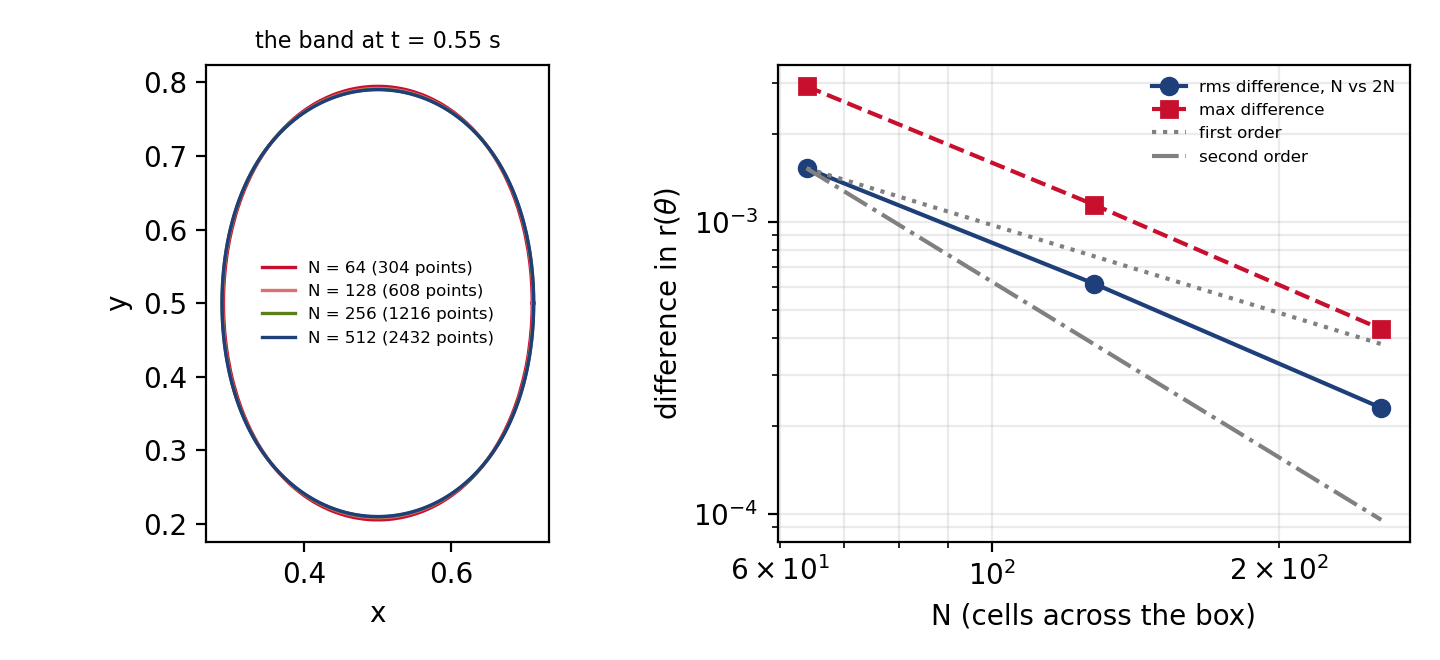
\includegraphics[width=\textwidth]{ch16-conv}
\vspace{1mm}

\scriptsize Left: the band at $t = 0.55$ s on the four grids. Right: the rms and maximum difference of the band's radius as a function of angle between each grid and the next finer one, against first- and second-order lines.
\end{column}
\end{columns}
\sourcecredit{IBAMR 0.19.0, \code{examples/IB/explicit/ex1}, inputs as shipped except \code{N}, the structure name and the position dumps; \code{tools/ch16\_conv.py}.}
\end{frame}

% 19
\begin{frame}{A convergence study (2): what the numbers say}
\label{fr:conv2}
\scriptsize The band starts as an ellipse of area $A$ and, incompressible fluid inside and out, must relax toward a circle of radius $\sqrt{A/\pi}$ while oscillating; at $t = 0.55$ s it is still oscillating, so the four shapes are compared with each other, not with the circle.
\vspace{1mm}

\scriptsize
\begin{center}
\begin{tabular}{@{}lllll@{}}
\toprule
grids & rms difference of $r(\theta)$ & max difference & mean radius & $(r_{\max} - r_{\min})/\bar r$\\
\midrule
$64$ & -- & -- & $0.2527$ & $0.336$\\
$64 \to 128$ & $1.53\times10^{-3}$ & $2.92\times10^{-3}$ & $0.2523$ & $0.320$\\
$128 \to 256$ & $6.16\times10^{-4}$ & $1.15\times10^{-3}$ & $0.2521$ & $0.313$\\
$256 \to 512$ & $2.31\times10^{-4}$ & $4.30\times10^{-4}$ & $0.2520$ & $0.311$\\
\midrule
observed order (rms; max) & $1.31$, then $1.41$ & $1.35$, then $1.42$ & & \\
\bottomrule
\end{tabular}
\end{center}
\scriptsize The band's radius as a function of angle moves by $1.5$ mm when the grid goes from $64$ to $128$ cells and by $0.6$ mm from $128$ to $256$ (on a band of radius $0.25$ m in a $1$ m box): the differences shrink by a factor $2.5$ per halving, an observed order of about $1.3$, between first and second. That is what the IB method does for a thin elastic interface: the velocity is continuous across the band but its derivative jumps, and the regularized delta function smears the jump over a few cells, so the error is first order there and second order away from it (chapter 5; Griffith and Peskin 2005). The mean radius converges to $0.2521$ ($0.1$ per cent between the first two grids, $0.04$ between the next); the circle of radius $0.25$ it is heading for is not yet reached because the band is still oscillating at $0.55$ s ($r_{\max} - r_{\min}$ is a third of the radius on every grid). The $512$ grid confirms it: the difference falls to $0.23$ mm and the order rises to $1.4$; the mean radius settles at $0.2520$, with the $64$ grid $2.7$ per cent and the $256$ grid $0.1$ per cent of the radius away from it in the rms sense.
\vspace{1mm}


\end{frame}

% 19b
\begin{frame}{A convergence study (3): three studies already in the tree}
\label{fr:conv3}
\footnotesize For when you want the official version:
\begin{itemize}\footnotesize
  \item \code{adv\_diff/ex0/converg2d}: a text file of results, not a script, from an advected--diffused lattice of Gaussians at $N = 16$ to $256$ against the exact solution: ``convergence rates: L1-norm: 1.9949 1.9989 1.9998 2.0000; L2-norm: 2.0000 \ldots'' for $\kappa = 0.1$, and still $1.99$ at $\kappa = 0.01$: the second-order scalar solver of chapter 24;
  \item \code{navier\_stokes/ex1/convergence\_tester.cpp}: a separate program that reads the hierarchy dumps of a coarse and a fine run of the same exact-solution flow (\code{hier\_dump\_interval}, or \code{coarse\_hier\_dump\_interval} and \code{fine\_hier\_dump\_interval} in \code{Main}) and prints the norms of their difference;
  \item IB/01's time-step study (chapter 5, the README): the band's shape the same to four digits for \code{DT} from $10^{-6}$ to $5\times10^{-4}$, and the abort at $10^{-3}$: convergence in time has a cliff, not a slope, once the step is stiffness-limited.
\end{itemize}
\end{frame}

% 20
\begin{frame}{How to do your own convergence study}
\label{fr:howto}
\footnotesize
\begin{enumerate}
  \item \al{Fix the problem.} Choose the dimensionless numbers (chapter 8b) and keep them: the same $\mathrm{Re}$, $k'$, $\mathrm{St}$ on every grid. Change nothing but the resolution.
  \item \al{Refine together.} Halve $\Delta x$ (\code{N}, or one more \code{MAX\_LEVELS}), regenerate the structure with $\Delta s = \Delta x/2$ (the generator's \code{N}), and halve \code{DT} if it is tied to the grid (it is, in every input of this series); three grids are the minimum for an order, four are better.
  \item \al{Pick a number.} Something the physics cares about and the output gives: a drag coefficient (chapter 11), a swimming speed (14), a radius or an amplitude (this chapter), the transport per period (9b). Not a picture.
  \item \al{Compare neighbours.} $e_N = |q_N - q_{2N}|$ between successive grids, or against the finest; the order is $p = \log_2(e_N/e_{2N})$. Expect about $2$ for smooth structures and $1$ where there are kinks, corners or thin boundaries with jumps across them (chapter 5), and less in time if the step is stiffness-limited.
  \item \al{Know when to stop.} When $e_N$ is below what you will claim, and when the next grid costs more than the question is worth: the $512$ grid of this study cost $19$ minutes against $28$ s at $64$ (the four ran at once on 16 ranks of one desktop PC, so the ratio, $40$, is the number that matters: eight times the cells and eight times the steps); in 3D each halving is sixteen times the cost (chapter 12).
  \item \al{Tighten the solver first} if the differences stall at a floor (slide \ref{fr:tol}), and check the dump interval: compare at the same \emph{time}, not the same step.
\end{enumerate}
\end{frame}

% 21
\begin{frame}{A debugging routine}
\label{fr:routine}
\vspace{-1.5mm}
\footnotesize When a run misbehaves, in this order; most problems are found before step 5.
\begin{enumerate}\footnotesize\setlength{\itemsep}{0pt}
  \item \al{Read the end of the log} and the screen output: an \code{Error message} block names the class and the reason (slides \ref{fr:table1}, \ref{fr:table1b}, \ref{fr:table2}); no message plus a segmentation fault means a null pointer or a missing writer (slide \ref{fr:silent}), or, at the first step of a restart, a dump written where a regrid was due (slide \ref{fr:table1b}).
  \item \al{Shorten the run} to 40 steps with viz every step and look at the first frames in VisIt (chapter 26): a structure that explodes at step 1 is a file or stiffness problem; one that drifts for hundreds of steps and then goes is a boundary-condition or contact problem.
  \item \al{Halve \code{DT}.} If the failure moves later or vanishes, it was the step. Then decide whether the stiffness or the step was wrong (slide \ref{fr:ramp}).
  \item \al{Remove things} until it works: one structure at a time, the forcing function, the update function, the boundary conditions (all periodic), the extra levels (\code{MAX\_LEVELS = 1}). What you put back last is the cause.
  \item \al{Count.} Vertices, springs, beams, targets in the log against the generator; the structure order in \code{structure\_names} against the indices the update functions use (chapters 8a, 9a, 9b).
  \item \al{Run in serial} (\code{-np 1}): a failure that depends on the number of ranks is a point crossing a patch boundary or a parallel-only code path.
  \item \al{Compare with the shipped example} it was copied from: run that, unchanged, and diff the inputs.
  \item \al{Then the tools}: a debug build (\code{-DCMAKE\_BUILD\_TYPE=Debug}, or autoibamr's \code{--prefix=\textasciitilde/autoibamr-debug} of chapter 2) under \code{gdb --args ./build/main2d input2d} gives a backtrace at the fault; PETSc's \code{-ksp\_monitor} and \code{-log\_view} show a solver that is struggling; \code{valgrind} finds the uninitialized value.
\end{enumerate}
\end{frame}

% 22
\begin{frame}{What can go wrong (1): the messages, collected}
\label{fr:table1}
\scriptsize
\setlength{\tabcolsep}{3pt}
\begin{tabular}{@{}L{0.38\textwidth}L{0.36\textwidth}L{0.22\textwidth}@{}}
\toprule
message & cause & chapter\\
\midrule
\code{Time step size change encountered. Aborting.} & the CFL-limited step fell below \code{DT}: an instability, a tearing structure, or a real fast transient & 5, 9b, 10, 13, 14; slide \ref{fr:cfl}\\
\code{IB point has escaped from the computational domain!} & a point crossed a non-periodic boundary, with \code{error\_if\_points\_leave\_domain = TRUE} in the \code{IBMethod} block (off by default) & 13; slide \ref{fr:soon}\\
\code{Structure X does not exist on level N} & \code{structure\_levels} and \code{level\_number} disagree, or a misspelt name & 14\\
\code{Update methods supported are CONSTRAINT\_VELOCITY, ...} & a bad \code{lag\_position\_update\_method} & 14\\
\code{frequency of cylinder does not exist in the InputDatabase} & a kinematics class's required key missing & 14\\
\code{incomplete beam curvature specification} & a \code{.beam} line with some but not \code{NDIM} curvature columns & 10\\
\bottomrule
\end{tabular}
\end{frame}

% 31b
\begin{frame}{What can go wrong (1): the messages, collected (2)}
\label{fr:table1b}
\scriptsize
\setlength{\tabcolsep}{3pt}
\begin{tabular}{@{}L{0.38\textwidth}L{0.36\textwidth}L{0.22\textwidth}@{}}
\toprule
message & cause & chapter\\
\midrule
\code{muParserRobinBcCoefs::} \code{setDataOnPatch()} error at step 1 & an expression muParser cannot read & 3, 7\\
a parse error with a line number & CRLF endings, curly quotes, \code{\%} comments, a missing brace & 3, 14; slide \ref{fr:parse}\\
\code{Example ... requires libMesh - skipping} & an IBFE or IIM example on an IBAMR without libMesh & 15\\
\code{physical domain must be a single box} & \code{domain\_boxes} with more than one box & 7\\
\code{Caught signal number 11 SEGV} at the first step of a restart, just after \code{regridding the patch hierarchy} & the dump was written at a step where a regrid was due (an IBAMR fault, seen in IBFE runs with 0.16.0 and 0.19.0): restart from another dump & 3, 17, 21\\
\bottomrule
\end{tabular}
\end{frame}

% 23
\begin{frame}{What can go wrong (2): the symptoms without a message}
\label{fr:table2}
\scriptsize
\setlength{\tabcolsep}{3pt}
\begin{tabular}{@{}L{0.3\textwidth}L{0.4\textwidth}L{0.26\textwidth}@{}}
\toprule
what you see & cause & chapter\\
\midrule
a segmentation fault at the first force evaluation & a spring force function index with no function registered & 9b\\
a segmentation fault at the first viz dump & \code{viz\_writer} without \code{"Silo"} in a program that registers the Silo writer & 13\\
nothing printed where output was expected & a \code{PrintOutput} or output key in the wrong block, or misspelt & 14\\
walls that meet and never reopen & no contact handling: points in one cell share a velocity & 9b, 14\\
a structure that does nothing & stiffness far too small for the grid and flow ($k'_{\mathrm{beam}} \ll 1$) & 10\\
a flickering velocity field & stiffness too high for the step & 9a, 10; slide \ref{fr:ramp}\\
all runs ten times slower than yesterday & several \code{mpirun} jobs bound to the same cores & 2\\
the disk full & viz or restart dumps every few steps for a long run & 9b, 14, 15\\
a Puma job that never starts, or stops early & an unsatisfiable request; the time, memory or quota limit & 1; slide \ref{fr:cluster}\\
the band drifts from its generator's shape at step 0 & the generator's \code{N} or \code{ds} and the input's grid disagree & 8a\\
\bottomrule
\end{tabular}
\vspace{1mm}

\scriptsize ``What can go wrong'' slides with the same table in short form: chapters 5, 6, 7, 8a, 8b, 9a, 9b, 10, 11, 12, 13, 14 and 15.
\end{frame}

% 24
\begin{frame}{Homework}
\label{fr:hw}
\footnotesize
\begin{enumerate}
  \item IB/01: raise \code{DT} until the run aborts, then set \code{warn\_on\_dt\_change = TRUE} and \code{error\_on\_dt\_change = FALSE} and run again; plot \code{dt} from the log against time and say what the integrator did instead of stopping.
  \item Run the two Python exercises of slides \ref{fr:exercises}--\ref{fr:exercises2} at the lecture's parameters and at one more of your own each; write the stability condition you observed as an inequality.
  \item Repeat the convergence study of slides \ref{fr:conv1}--\ref{fr:conv2} on IB/03 (chapter 8a's tethered beam) with the drag coefficient of chapter 11 as the number: three grids, one order.
  \item Take the upstream cylinder of chapter 15 (\code{IB/explicit/ex2}) and set \code{vorticity\_rel\_thresh} to $0.5$, $0.25$ and $0.1$; count the finest-level cells in the log at $t = 20$ s and compare the wake in VisIt.
  \item Make a run fail on purpose in three different ways (a key in the wrong block, a point outside the box, a stiffness ten times too high) and write down, for each, the first line of the log that gave it away.
\end{enumerate}
\end{frame}

% 25
\begin{frame}{Rules of thumb}
\label{fr:thumb}
\small
\begin{itemize}
  \item \code{grep "dt = " IB2d.log} first; \code{integral\{F\}} second.
  \item ``Time step size change'' means the fluid got faster than \code{DT} allows; find out why before loosening the check.
  \item Ramp every start; match the step to the stiffness, not the stiffness to the step.
  \item Refine where the vortices are: \code{vorticity\_rel\_thresh} or \code{\_abs\_thresh}, \code{tag\_buffer}.
  \item Tighten the solver when a conserved quantity drifts; it costs iterations, not accuracy.
  \item Match $\mathrm{Re}$, $k'$, $\mathrm{St}$, $\mathrm{Wo}$ together, and $\mathrm{St} = fL/U$.
  \item Walls do not touch, points do not leave, keys sit in the right block.
  \item Three grids, one number, one order; the step refined with the grid.
  \item Shorten, halve, remove, count, serialize, compare, then \code{gdb}.
\end{itemize}
\end{frame}

% 26
\begin{frame}{Summary}
\label{fr:summary}
\footnotesize
\begin{enumerate}
  \item IBAMR's loudest failure, the time-step-change abort, is a CFL check on a fixed step; its usual causes in Part III were a step too large for a stiffness, a structure driven into itself or into a step, and a real transient. Watching \code{dt} in the log, as the 2012 ReadMe said, still catches it earliest.
  \item The 2014 rules stand, with their keys verified: ramp the start, keep the stiffness and the step consistent, refine by vorticity thresholds in the integrator's block, tighten the Stokes solver by its sub-block (or the old \code{-stokes\_ksp\_rtol}), and match every dimensionless number; the Strouhal number and the 2D bending stiffness are corrected.
  \item The promised ``other points'' are written: walls touching stick, a net inflow has no solution, oscillations have numerical and physical kinds, and a point leaving the box is caught by a named message only if the check is switched on.
  \item Convergence means the number you care about stops changing as the grid and the step are refined together; the bouncing band gives an observed order of $1.3$ to $1.4$ across the $64$, $128$, $256$ and $512$ grids, IBAMR's own scalar study gives second order, and the time-step study of IB/01 shows a cliff.
  \item When a run misbehaves: read, shorten, halve, remove, count, serialize, compare, debug, in that order.
\end{enumerate}
\begin{homebox}
\footnotesize This closes Part III. Part IV, chapters 17 to 25, is the finite-element method, IBFE.
\end{homebox}
\end{frame}

% 27
\begin{frame}{What changed since the older course notes}
\label{fr:changed}
\footnotesize
\begin{itemize}
  \item The 2014 deck's five rules are quoted and each checked against 0.19.0: both vorticity keys exist (with the block and the per-level form stated), the \code{stokes\_} prefix survives and the input-file form is given, the Strouhal number and the 2D bending exponent are corrected, and the MATLAB-style snippet is marked as unparseable.
  \item Its ``other points coming soon'' are written from the series' own runs.
  \item The 2021 lecture's definitions and exercises are kept, its IB2d lab is mapped to IBAMR, and its claim that the CFL condition rarely matters in IB is qualified with where IBAMR applies one.
  \item The convergence study is new: four grids of an upstream example with measured differences and an order; the three studies already in the tree are pointed out.
  \item The 2019 cluster tips are translated to Puma and their two inaccuracies named; the debugging routine and the two tables are new, with every message traced to the source or to a chapter.
\end{itemize}
\end{frame}

% 28
\begin{frame}{Recordings (listed, not incorporated)}
\label{fr:videos}
\small The 2014 \emph{What can go wrong} tutorial has no recording. The 2021 MATH 481 Lecture 19 was given in class with a VCAT (remote desktop) session for the MATLAB exercises; no recording is in the course's folders. Nothing from a recording is reproduced here.
\end{frame}

% 29
\begin{frame}{References}
\label{fr:refs}
\scriptsize
\begin{itemize}
  \item IBAMR 0.19.0: \code{src/IB/IBHierarchyIntegrator.cpp} (the dt-change check and keys), \code{src/navier\_stokes/INSHierarchyIntegrator.cpp} (vorticity thresholds), \code{src/navier\_stokes/INSStaggeredHierarchyIntegrator.cpp} (the Stokes solver and its prefix), \code{ibtk/src/lagrangian/LDataManager.cpp} (the escaped point), \code{ibtk/src/solvers/impls/PETScKrylovLinearSolver.cpp} (tolerance keys), \code{examples/IB/explicit/ex1}, \code{examples/adv\_diff/ex0/converg2d}, \code{examples/navier\_stokes/ex1/convergence\_tester.cpp}. \url{https://github.com/IBAMR/IBAMR}
  \item C. S. Peskin, \emph{The immersed boundary method}, Acta Numerica 11 (2002) 479--517 (accuracy of the method); B. E. Griffith and C. S. Peskin, \emph{On the order of accuracy of the immersed boundary method: higher order convergence rates for sufficiently smooth problems}, J.\ Comput.\ Phys.\ 208 (2005) 75--105.
  \item This series: \code{examples/support/matlab-exercises} (\code{stiff\_ode\_example}, \code{heat\_equation}, MATLAB and Python), \code{tools/ch16\_conv.py}, IB/01's README (the time-step table), chapter 3's error table.
  \item Sources: \emph{11-IBAMR Tutorial: What can go wrong} (2014, 14 slides); \emph{MATH 481 Lecture 19: Stability and convergence} (2021, edited 2023, 40 slides); the lab ReadMe deck (2012), slide 5; \emph{Debugging tips} (2019, 4 slides, also slides 13--16 of the 2018--20 Dogwood deck).
\end{itemize}
\end{frame}

\end{document}
